\section{Results}

First weeks were dedicated to implement, optimize and test the Monte Carlo simulation code. Reaching an efficient and accurate code was essential before studying the polycrystalline model and it was a challenging task. Systems studied need a lot of Monte Carlo steps to reach equilibrium near transition. Optimize and parallelize the code was then very important and it took some time.

The first part of the results section focuses on validating the Monte Carlo simulation code by applying it to the well-known XY model. After that, the polycrystalline model is studied to know if the system can be described by the KTHNY theory.

\subsection{Validation on the XY model}

The first step was to validate the Monte Carlo simulation code by applying it to the classical XY model, which is a well-studied system. The Hamiltonian of the XY model is given by:
\begin{equation}
    \mathcal{H}_{XY} = -J \sum_{\langle i,j \rangle} \cos(\theta_i - \theta_j)
\end{equation}

Where $J$ is the coupling constant, $J = 1$ for the rest of this part. The geometry used is the same hexagonal lattice as in the polycrystalline model. The thermodynamic behavior of the XY model is characterized by a Berezinskii-Kosterlitz-Thouless (BKT) \cite{Kosterlitz1973} transition at a critical temperature $T_{BKT}$. Below this temperature, the system exhibits quasi-long-range order, while above it, the system is disordered. According to Sorokin \cite{Sorokin2019}, who studied different lattice geometries, the critical temperature for the XY model on a triangular lattice is approximately $T_{BKT} = 1.418$. The correlation function $G(r)$ was computed and the exponent $\eta(T)$ was extracted to find the transition temperature where $\eta(T_{BKT}) = 1/4$. Simulations were run for lattice sizes $L = 16, 32, 64$ and for temperatures ranging from $T = \num{1e-5}$ to $T = 2.0$. Correlation functions for $L = 64$ and their fits are shown in \cref{fig:correlation_XY}. The extracted exponent $\eta(T)$ as a function of temperature is shown in \cref{fig:XY_eta_vs_T}. Finally, the susceptibility $\chi$ as a function of temperature for different lattice sizes is shown in \cref{fig:XY_chi_vs_L}. Results are in good agreement with the expected behavior of the XY model. With the critical exponent condition $\eta(T_{BKT}) = 1/4$, the transition temperature is found to be $T_{BKT} = 1.42 \pm 0.03$, which is consistent with the value in the literature. Additionally, the susceptibility $\chi$ shows a peak just above the transition temperature, which becomes more pronounced with increasing lattice size, as expected. Under the critical temperature, the system exhibits quasi-long-range order, while above it, the system decays exponentially, confirming the disordered phase. At $T = \num{1e-5}$, the system is nearly perfectly ordered. 

Under these observations, the Monte Carlo simulation code is validated for the XY model and can be used to study the polycrystalline model.

\begin{figure}[htbp]
    \centering

    \begin{subfigure}[t]{0.47\textwidth}
        \centering
        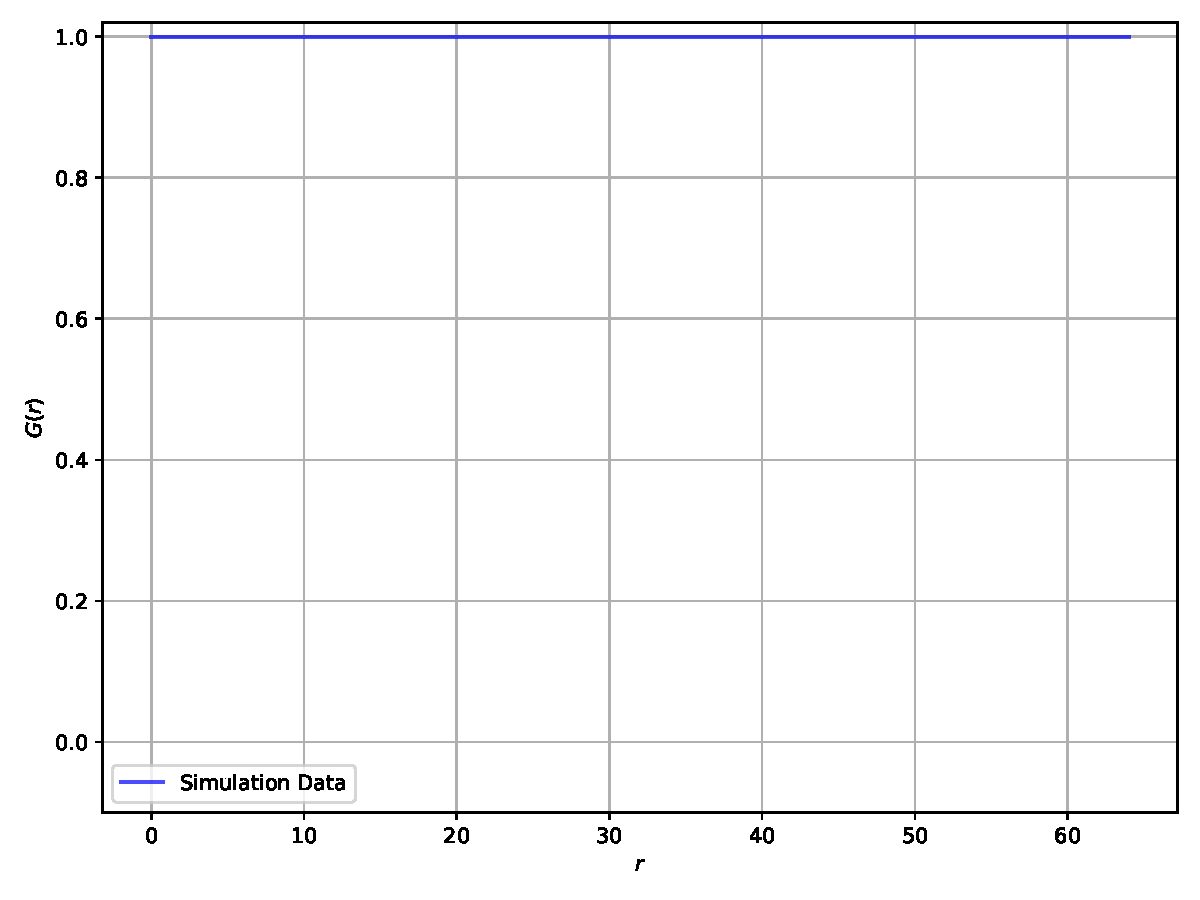
\includegraphics[width=\textwidth]{Figures/XY/correlation_T1.000e-05_L64.pdf}
        \caption{$T = \num{1e-5}$}
    \end{subfigure}
    \hfill
    \begin{subfigure}[t]{0.47\textwidth}
        \centering
        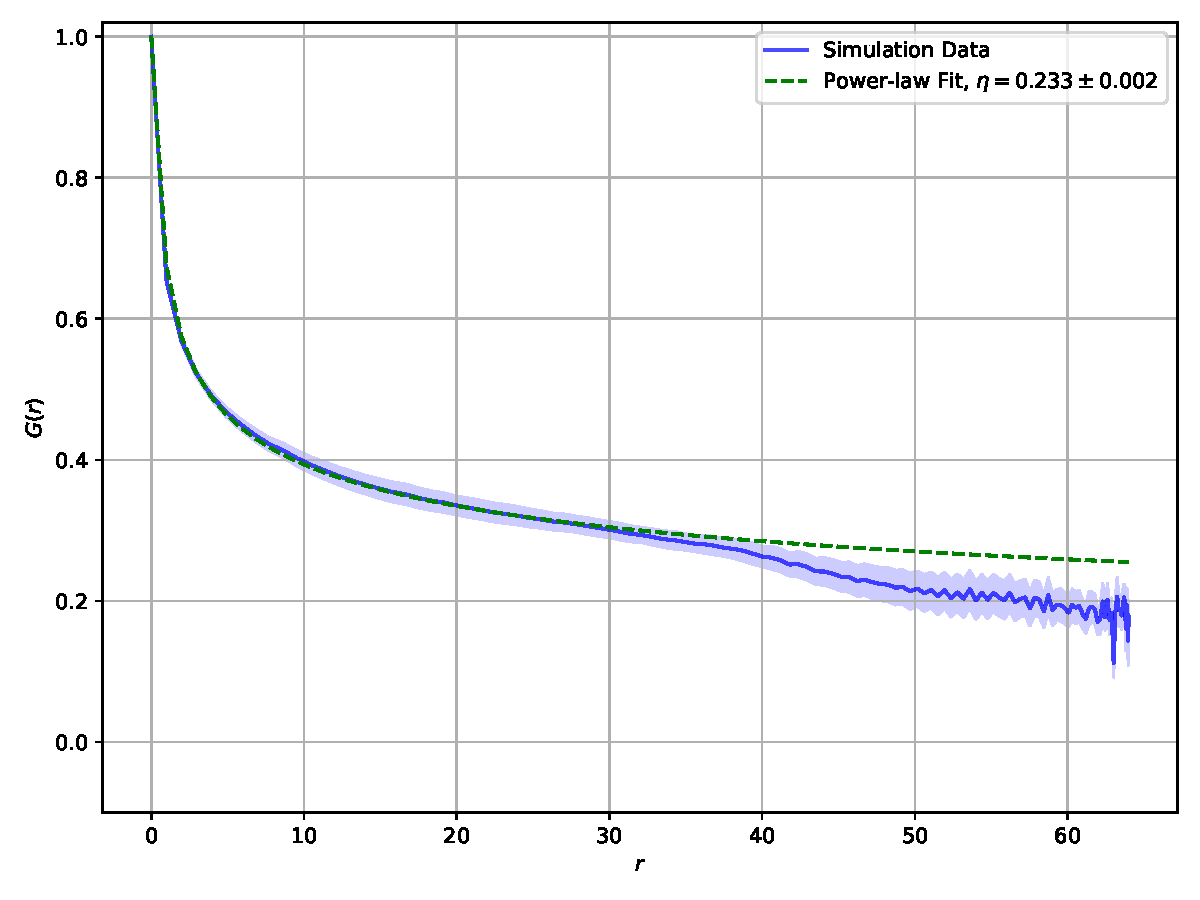
\includegraphics[width=\textwidth]{Figures/XY/correlation_T1.400e+00_L64.pdf}
        \caption{$T = 1.4$}
    \end{subfigure}

    \medskip

    \begin{subfigure}[t]{0.47\textwidth}
        \centering
        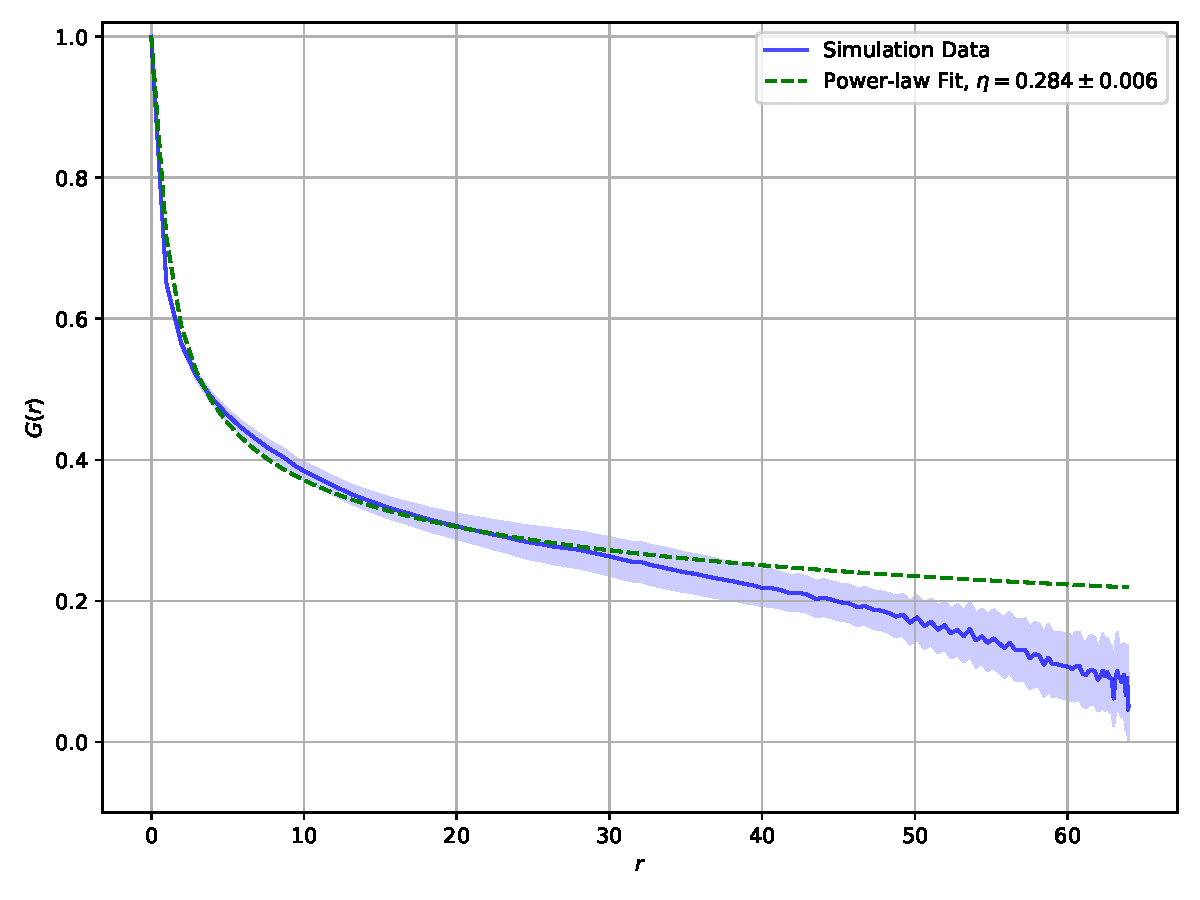
\includegraphics[width=\textwidth]{Figures/XY/correlation_T1.420e+00_L64.pdf}
        \caption{$T = 1.42$}
    \end{subfigure}
    \hfill
    \begin{subfigure}[t]{0.47\textwidth}
        \centering
        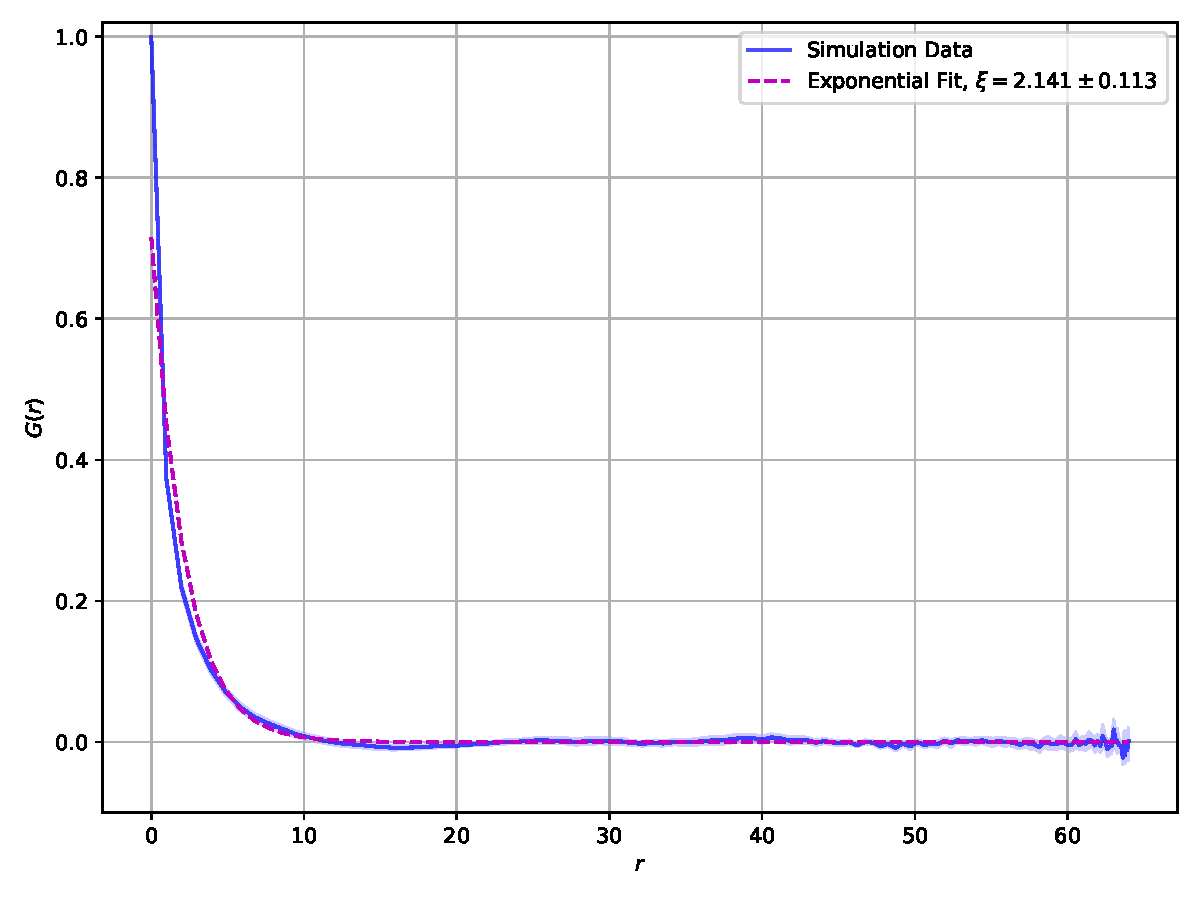
\includegraphics[width=\textwidth]{Figures/XY/correlation_T2.000e+00_L64.pdf}
        \caption{$T = 2.0$}
    \end{subfigure}
    \caption{Correlation functions of the XY model at different temperatures with lattice size $L = 64$.}
    \label{fig:correlation_XY}
\end{figure}

\begin{figure}[htbp]
    \centering

    \begin{subfigure}[t]{0.47\textwidth}
        \centering
        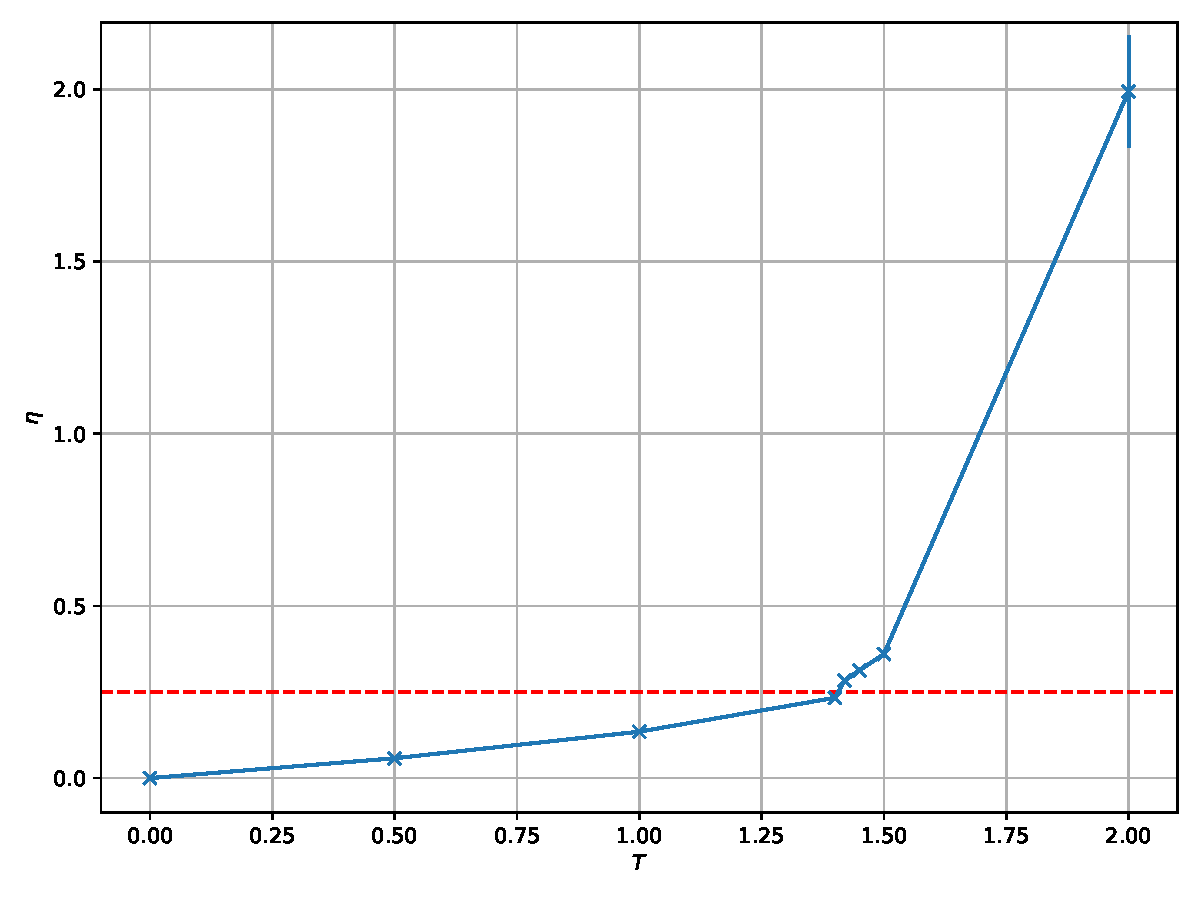
\includegraphics[width=\textwidth]{Figures/XY/eta_L64.pdf}
        \caption{$\eta$}
        \label{fig:XY_eta_vs_T}        
    \end{subfigure}
    \hfill
    \begin{subfigure}[t]{0.47\textwidth}
        \centering
        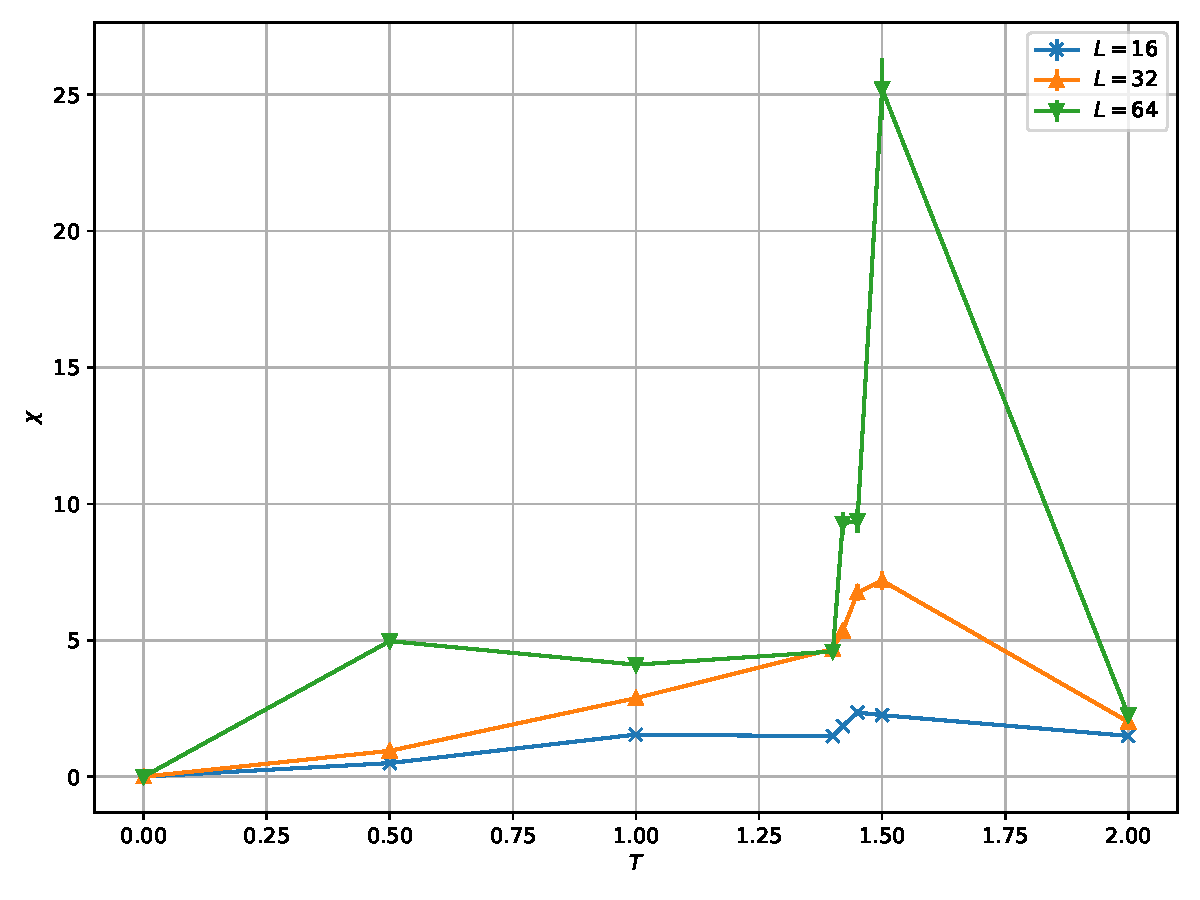
\includegraphics[width=\textwidth]{Figures/XY/chi_vs_T_all_L.pdf}
        \caption{$\chi$}
        \label{fig:XY_chi_vs_L}
    \end{subfigure}
    \caption{Exponent $\eta$ and susceptibility $\chi$ of the XY model as a function of the temperature for $L = 64$, respectively, $L = 16, 32, 64$.}
\end{figure}

\FloatBarrier

\subsection{Polycrystalline Model without Grain Interactions}

The first step was to verify the crystalline order of the system when there is no interaction between grains, i.e., $\gamma = 0$ and $\epsilon = 1$. Simulations were run for $L = 16, 32, 64$ and for temperatures ranging from $T = \num{1e-5}$ to $T = 1.0$. The measured correlation functions and their theoretical predictions are shown in \cref{fig:correlation_eps1_gamma0} for $L = 64$. The susceptibility $\chi_6$ as a function of the inverse lattice size $L^{-1}$ is shown in \cref{fig:chi_eps1_gamma0}. These results confirm that when there is no interaction between grains, the system behaves like a perfect crystal until it reaches a totally disordered state at high temperatures. Correlation functions match the theoretical predictions calculated with \cref{eq:theoricG6}, and the susceptibility $\chi_6$ remains constant with increasing lattice size, indicating long-range order or total disorder.

\begin{figure}[htbp]
    \centering
    
    \begin{subfigure}[t]{0.47\textwidth}
        \centering
        
\includegraphics[width=\textwidth]{Figures/eps1/correlation_T1.000e-05_L64.pdf}
        \caption{$T = \num{1e-5}$}
    \end{subfigure}
    \hfill
    \begin{subfigure}[t]{0.47\textwidth}
        \centering
        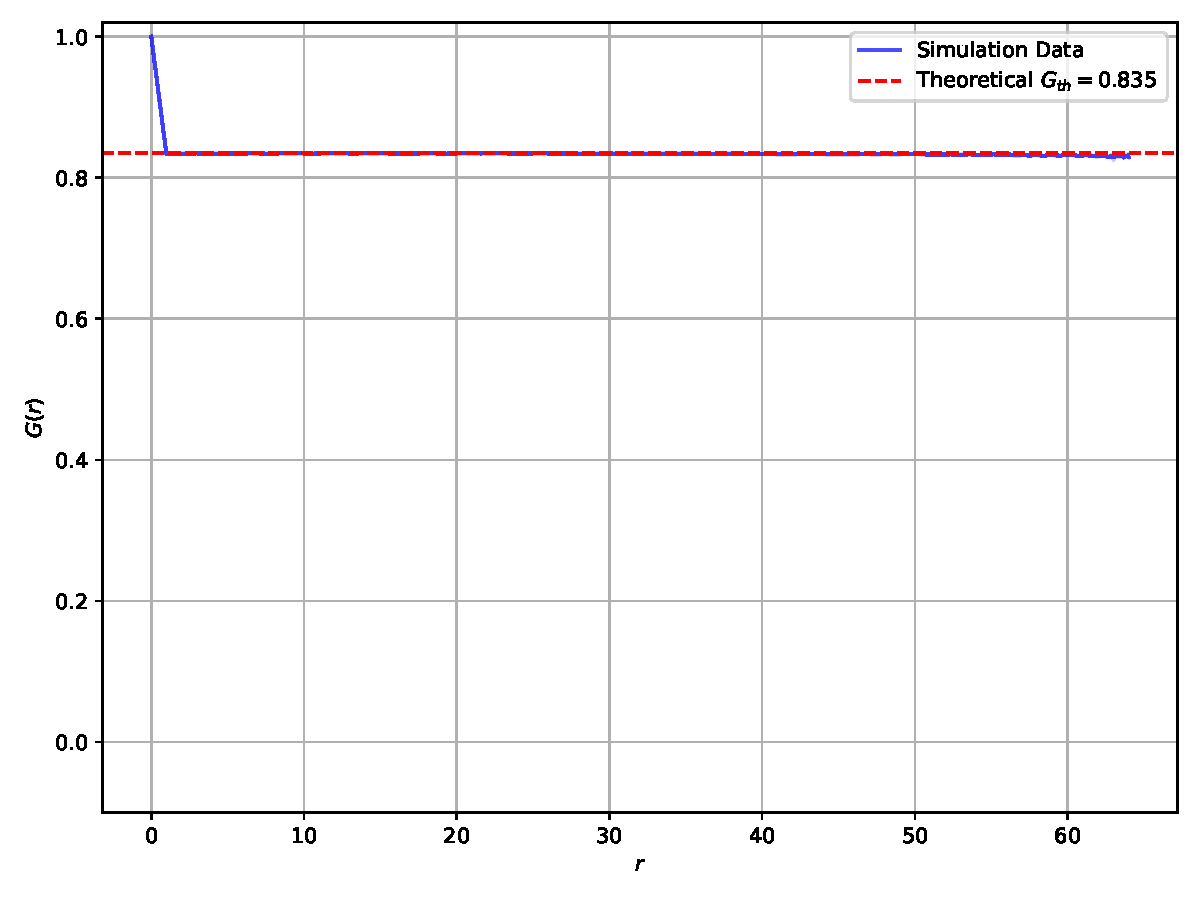
\includegraphics[width=\textwidth]{Figures/eps1/correlation_T1.000e-02_L64.pdf}
        \caption{$T = 0.01$}
    \end{subfigure}

    \medskip

    \begin{subfigure}[t]{0.47\textwidth}
        \centering
        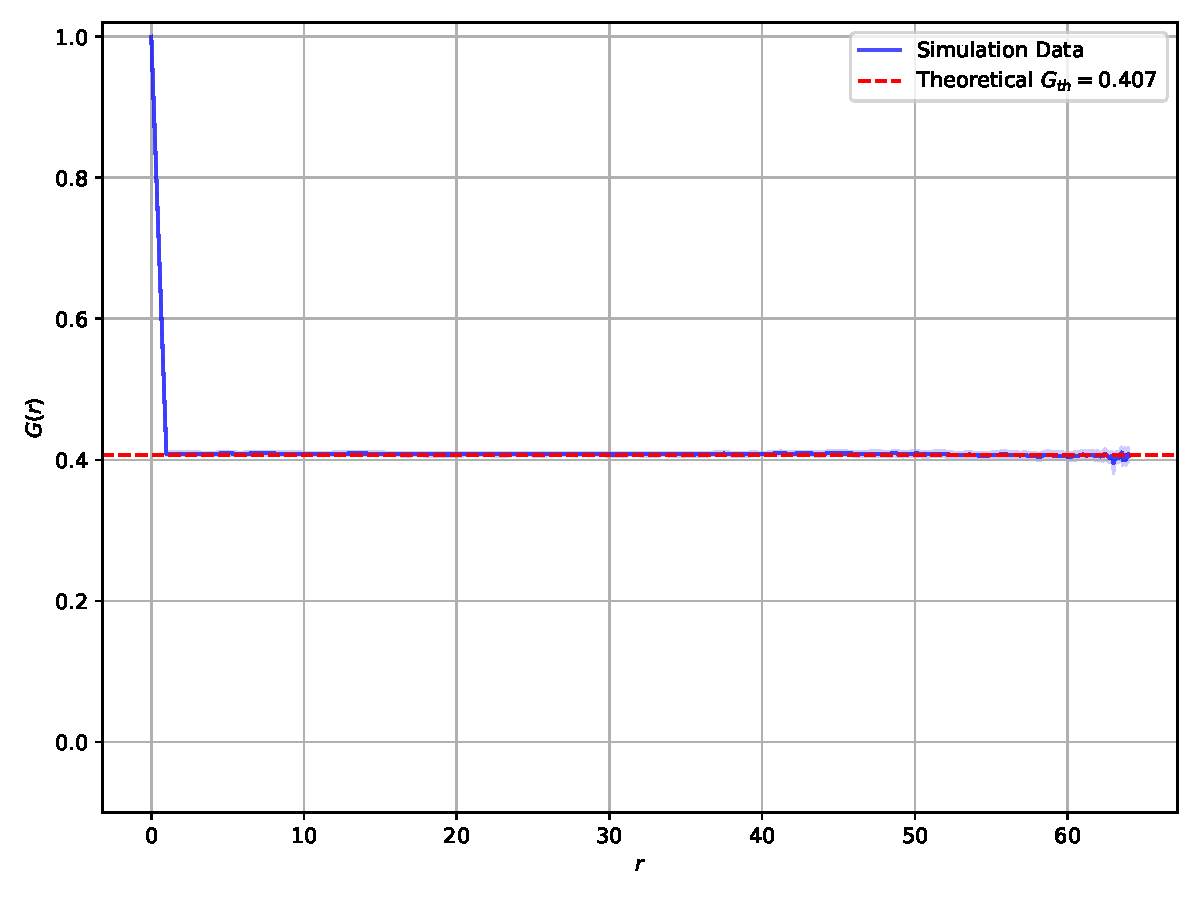
\includegraphics[width=\textwidth]{Figures/eps1/correlation_T5.000e-02_L64.pdf}
        \caption{$T = 0.05$}
    \end{subfigure}
    \hfill
    \begin{subfigure}[t]{0.47\textwidth}
        \centering
        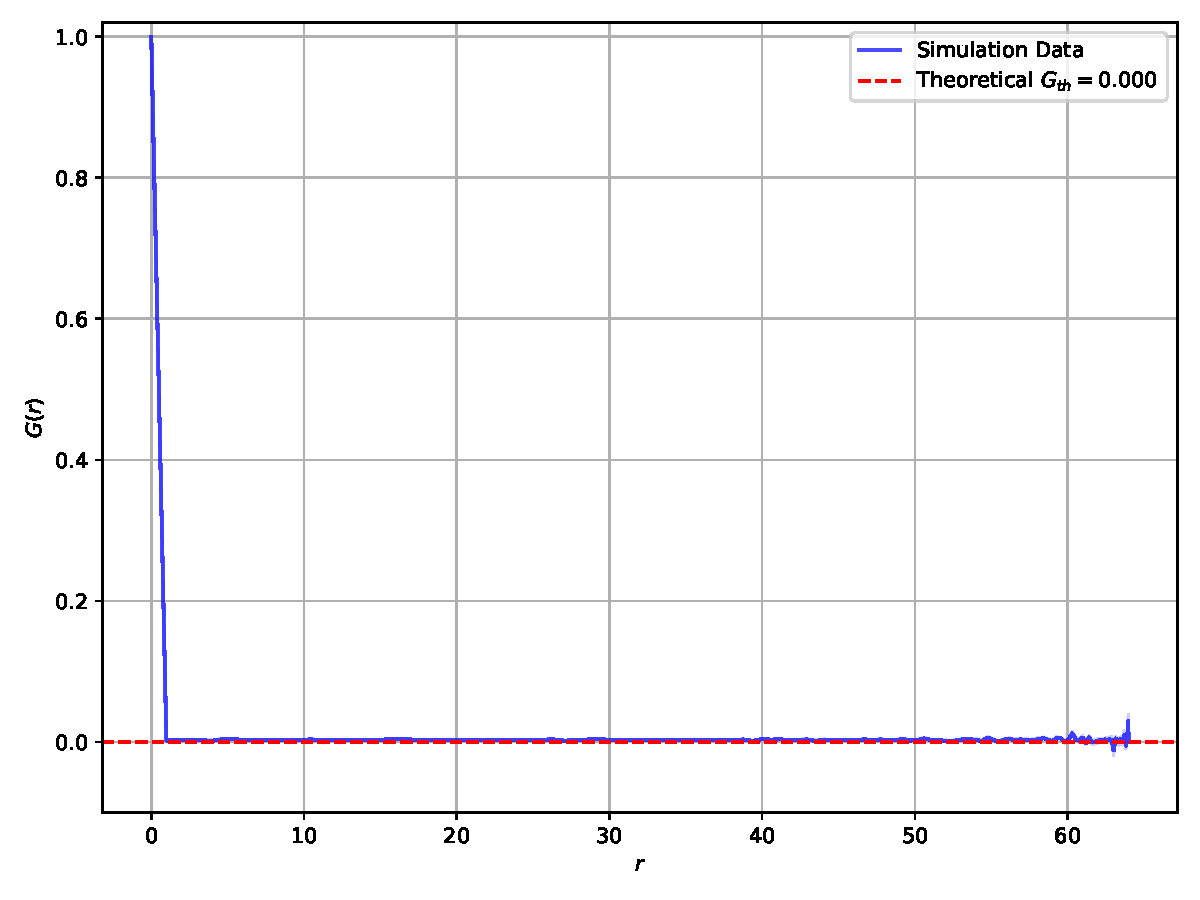
\includegraphics[width=\textwidth]{Figures/eps1/correlation_T1.000e+00_L64.pdf}
        \caption{$T = 1.0$}
    \end{subfigure}

    \caption{Correlation functions for the polycrystalline model with $\epsilon = 1.0$ and $\gamma = 0.0$ at different temperatures with lattice size $L = 64$.}
    \label{fig:correlation_eps1_gamma0}
\end{figure}

\begin{figure}[htbp]
    \centering
    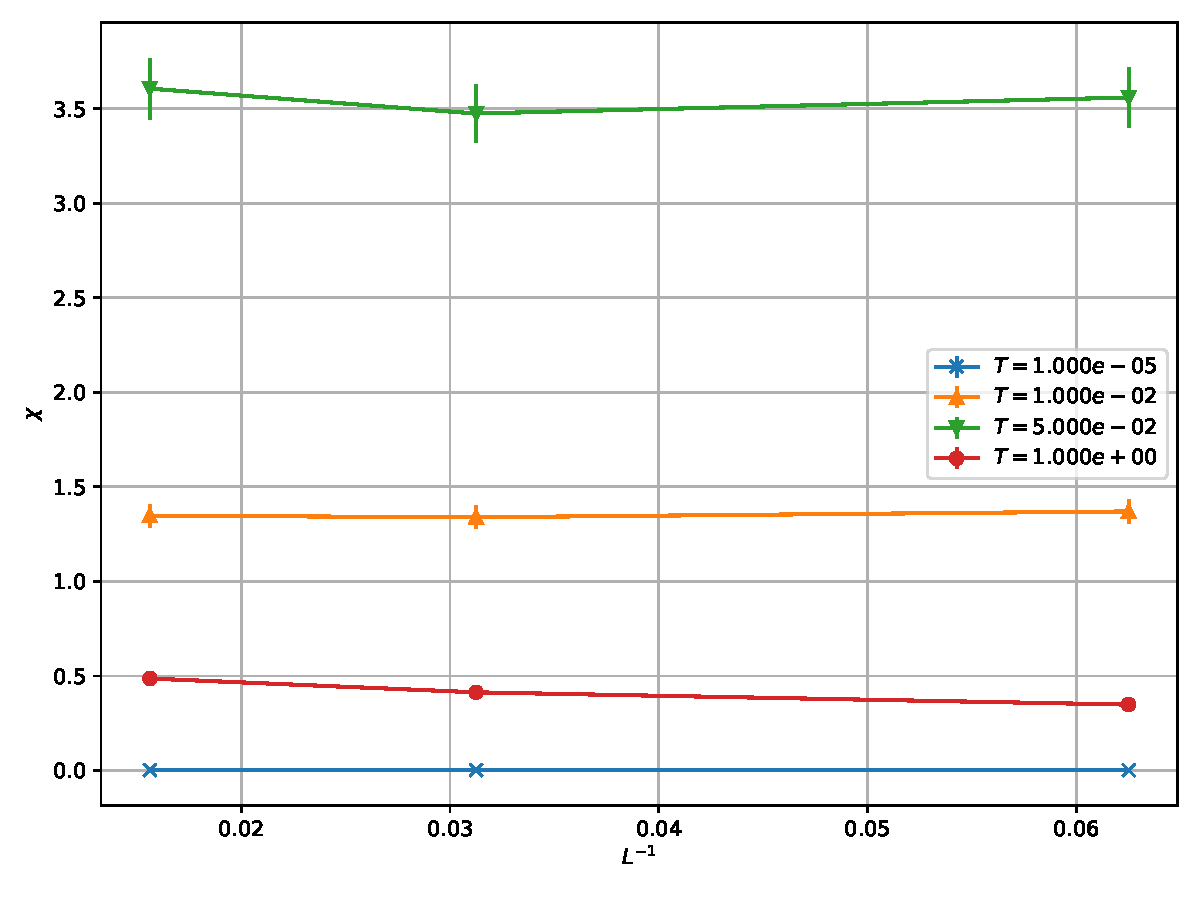
\includegraphics[width=0.47\textwidth]{Figures/eps1/chi_vs_L.pdf}
    \caption{Susceptibility $\chi_6$ as a function of the inverse lattice size $L^{-1}$ for the polycrystalline model with $\epsilon = 1.0$ and $\gamma = 0.0$ at different temperatures.}
    \label{fig:chi_eps1_gamma0}
\end{figure}

\FloatBarrier

\subsection{Polycrystalline Model with Grain Interactions}

The system was then studied with grain interactions, setting $\gamma = 1.0$ and $\epsilon = 0.0$. Simulations were run for $L = 16, 32, 64, 128, 256$ and for temperatures ranging from $T = \num{1e-5}$ to $T = 0.3$. The measured correlation functions for $L = 256$ and their fits are shown in \cref{fig:correlation_eps0_gamma1} for different temperatures. To compare the configuration in different phases, final lattices of each temperature are shown in \cref{fig:lattices_eps0_gamma1}. The extracted exponent $\eta_6(T)$ as a function of temperature is shown in \cref{fig:eta_eps0_gamma1}. The susceptibility $\chi_6$ as a function of temperature for different lattice sizes is shown in \cref{fig:chi_T_eps0_gamma1}. Finally, the susceptibility $\chi_6$ as a function of the inverse lattice size $L^{-1}$ at different temperatures near the transition and far from the transition is shown in \cref{fig:chi_L_eps0_gamma1}. Results indicate that the system undergoes a phase transition consistent with a BKT transition. The correlation functions show a change from a power-law decay to an exponential decay as the temperature increases. The exponent $\eta_6$ reaches the critical value of $1/4$ at a transition temperature of $T = 0.195 \pm 0.005$. The susceptibility $\chi_6$ exhibits a peak right above the transition temperature, which becomes more pronounced with increasing lattice size. At temperatures near the transition, the susceptibility increases exponentially with lattice size, while far from the transition, it remains relatively constant, indicating a transition to a disordered phase. The use of open boundary conditions introduce some finite-size effects, but the overall behavior is consistent with expectations for a BKT transition. To avoid these effects, larger lattice sizes are necessary but they require significantly more computational resources.

These findings support the applicability of the KTHNY theory to this polycrystalline model with grain interactions. However, the results are not very accurate yet, and further investigations with larger lattice sizes and more temperatures are needed to confirm these observations and refine the estimates of critical exponents and transition temperatures. Additionally, the existence of the hexatic phase between the ordered and disordered phases should be examined at higher lattice sizes with more thermalization steps to study attentively the behavior of the correlation functions at large distances.

The influence of the substrate coupling strength $\epsilon$ on the phase behavior should also be explored in future work to see how the competition between substrate coupling and grain interactions affects the phase transition. Parameters $A$ and $\rho$ in the Hamiltonian could also be varied to study their impact on the system's behavior.

\begin{figure}[htbp]
    \centering

    \begin{subfigure}[t]{0.47\textwidth}
        \centering
        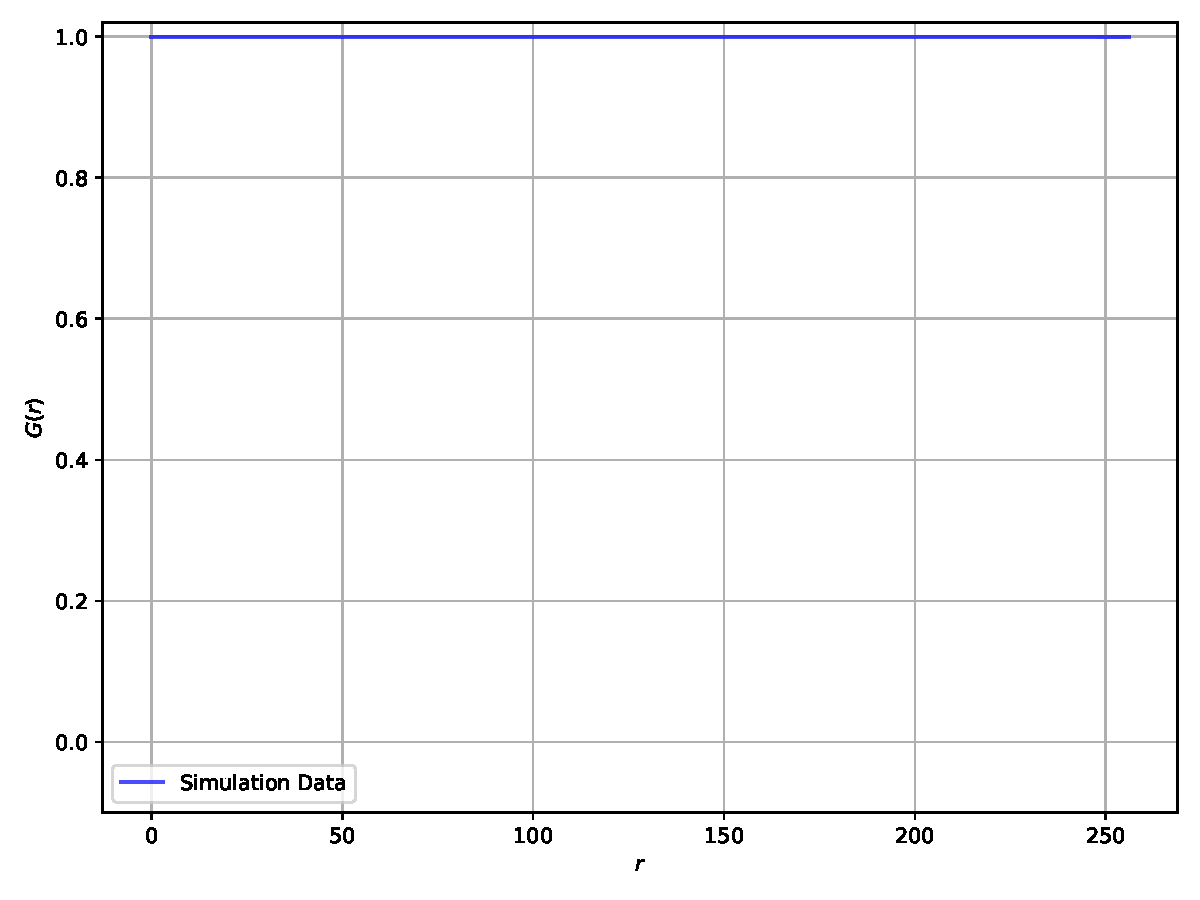
\includegraphics[width=\textwidth]{Figures/gamma1/correlation_T1.000e-02_L256.pdf}
        \caption{$T = 0.01$}
    \end{subfigure}
    \hfill
    \begin{subfigure}[t]{0.47\textwidth}
        \centering
        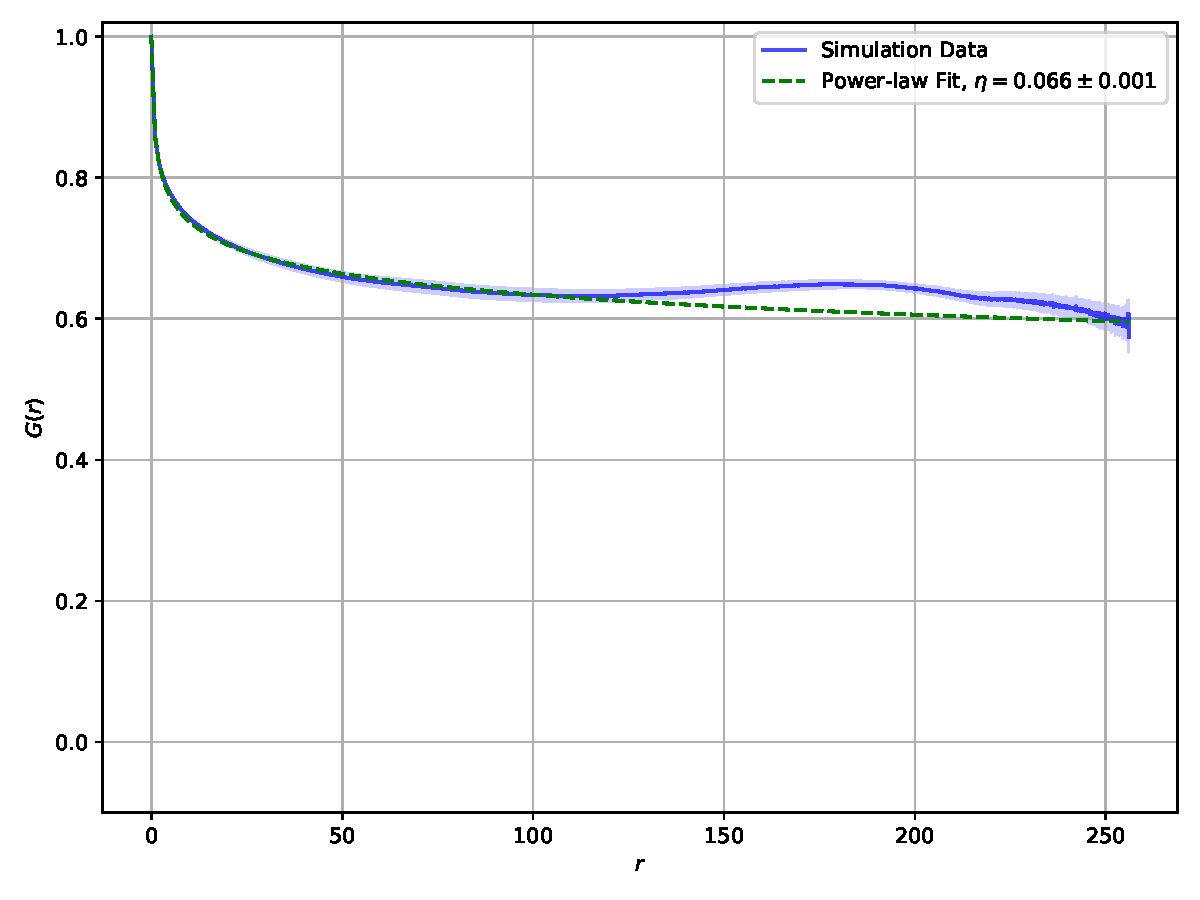
\includegraphics[width=\textwidth]{Figures/gamma1/correlation_T1.500e-01_L256.pdf}
        \caption{$T = 0.15$}
    \end{subfigure}

    \medskip

    \begin{subfigure}[t]{0.47\textwidth}
        \centering
        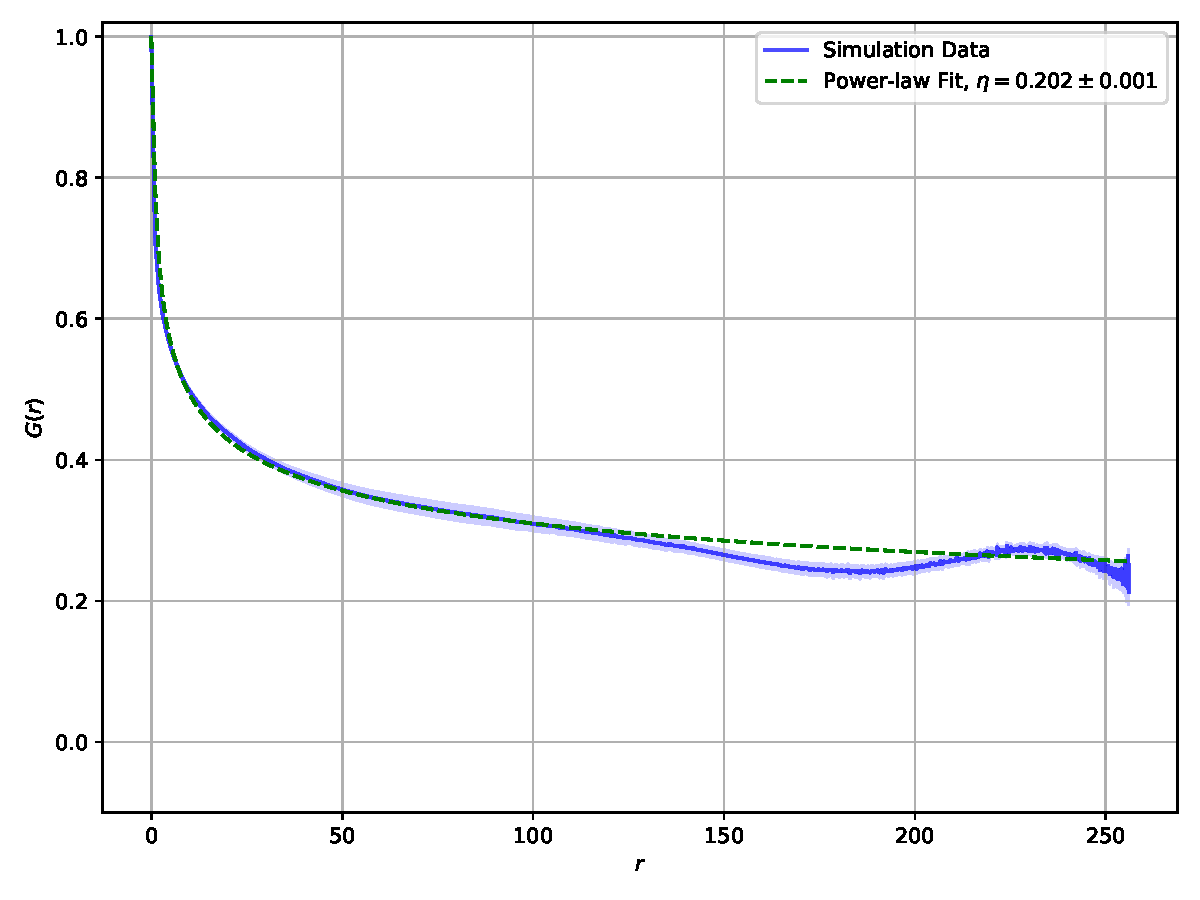
\includegraphics[width=\textwidth]{Figures/gamma1/correlation_T1.850e-01_L256.pdf}
        \caption{$T = 0.185$}
    \end{subfigure}
    \hfill
    \begin{subfigure}[t]{0.47\textwidth}
        \centering
        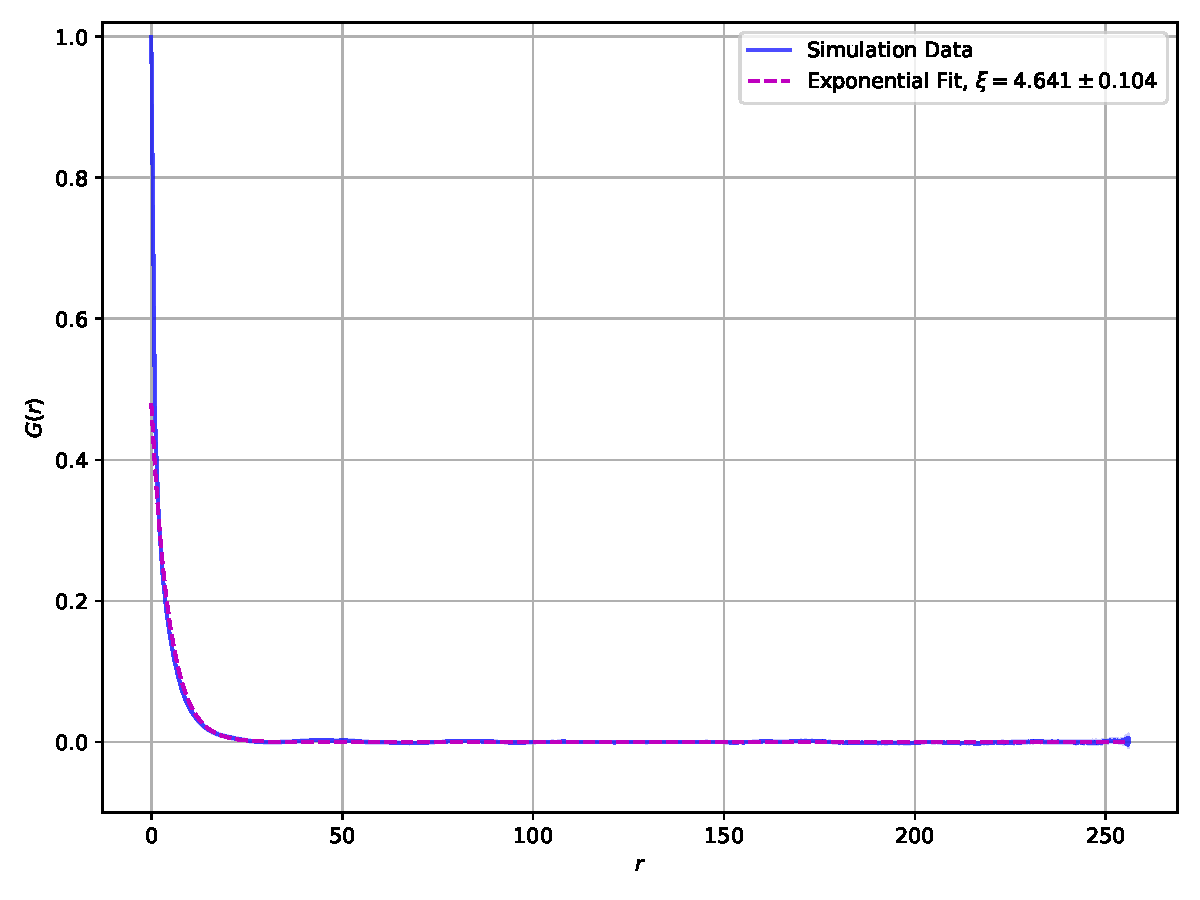
\includegraphics[width=\textwidth]{Figures/gamma1/correlation_T2.200e-01_L256.pdf}
        \caption{$T = 0.22$}        
    \end{subfigure}
    \caption{Correlation functions for the polycrystalline model with $\epsilon = 0.0$ and $\gamma = 1.0$ at different temperatures with lattice size $L = 256$.}
    \label{fig:correlation_eps0_gamma1}    
\end{figure}

\begin{figure}[htbp]
    \centering
    \begin{subfigure}[t]{0.47\textwidth}
        \centering
        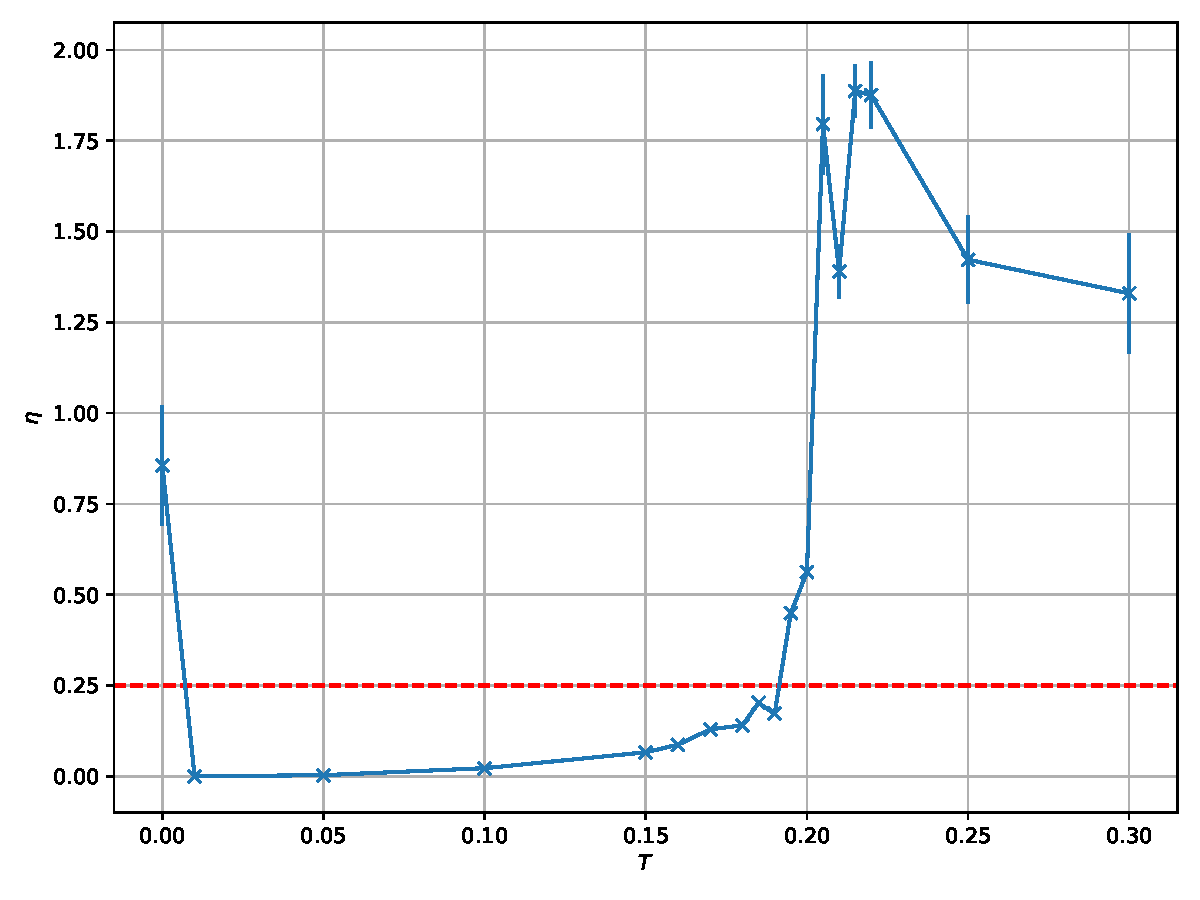
\includegraphics[width=\textwidth]{Figures/gamma1/eta_L256.pdf}
        \caption{$\eta_6$}
        \label{fig:eta_eps0_gamma1}        
    \end{subfigure}
    \hfill
    \begin{subfigure}[t]{0.47\textwidth}
        \centering
        
\includegraphics[width=\textwidth]{Figures/gamma1/chi_vs_T_all_L.pdf}
        \caption{$\chi_6$}
        \label{fig:chi_T_eps0_gamma1}
    \end{subfigure}
    \caption{Exponent $\eta_6$ and susceptibility $\chi_6$ of the polycrystalline model with $\epsilon = 0.0$ and $\gamma = 1.0$ as a function of the temperature for $L = 256$, respectively, $L = 16, 32, 64, 128, 256$.}
\end{figure}

\begin{figure}[htbp]
    \centering

    \begin{subfigure}[t]{0.47\textwidth}
        \centering
        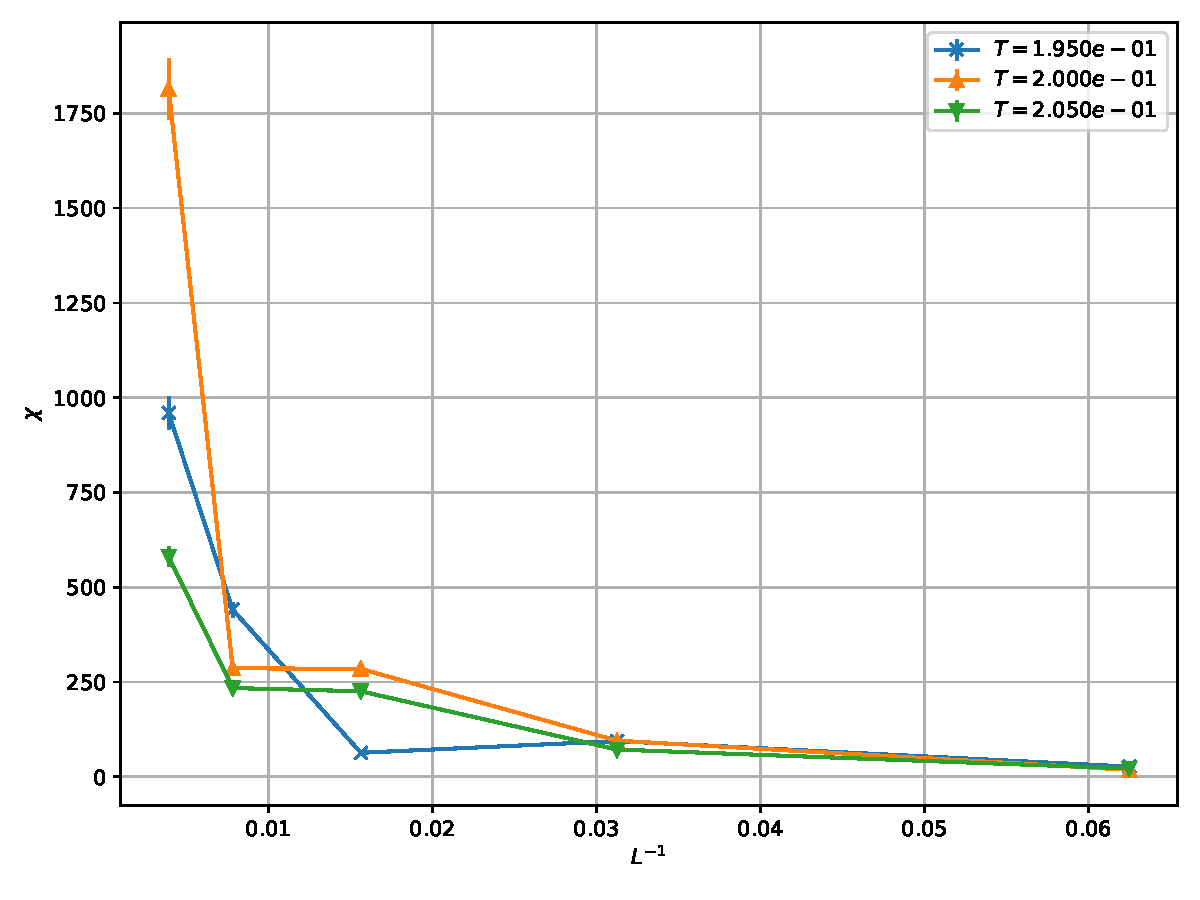
\includegraphics[width=\textwidth]{Figures/gamma1/chi_vs_L_transition.pdf}
        \caption{$\chi_6$ at transition}
        \label{fig:chi_L_transition_eps0_gamma1}
    \end{subfigure}
    \hfill
    \begin{subfigure}[t]{0.47\textwidth}
        \centering
        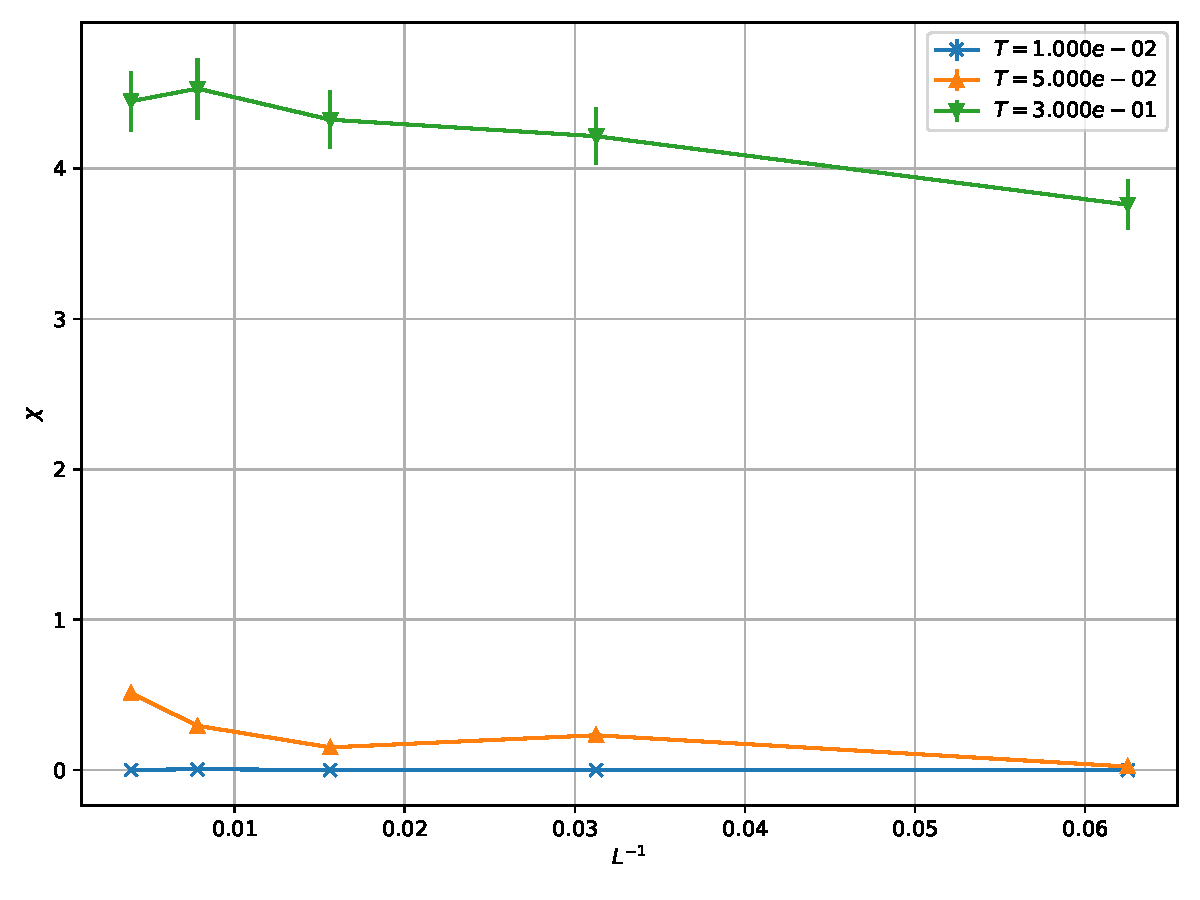
\includegraphics[width=\textwidth]{Figures/gamma1/chi_vs_L_0.pdf}
        \caption{$\chi_6$ not at transition}
        \label{fig:chi_L_no_transition_eps0_gamma1}
    \end{subfigure}
    \caption{Susceptibility $\chi_6$ as a function of the inverse lattice size $L^{-1}$ for the polycrystalline model with $\epsilon = 0.0$ and $\gamma = 1.0$ at different temperatures near the transition (a) and far frsom the transition (b).}
    \label{fig:chi_L_eps0_gamma1}
\end{figure}

\begin{figure}[htbp]
    \centering

    \begin{subfigure}[t]{0.495\textwidth}
        \centering
        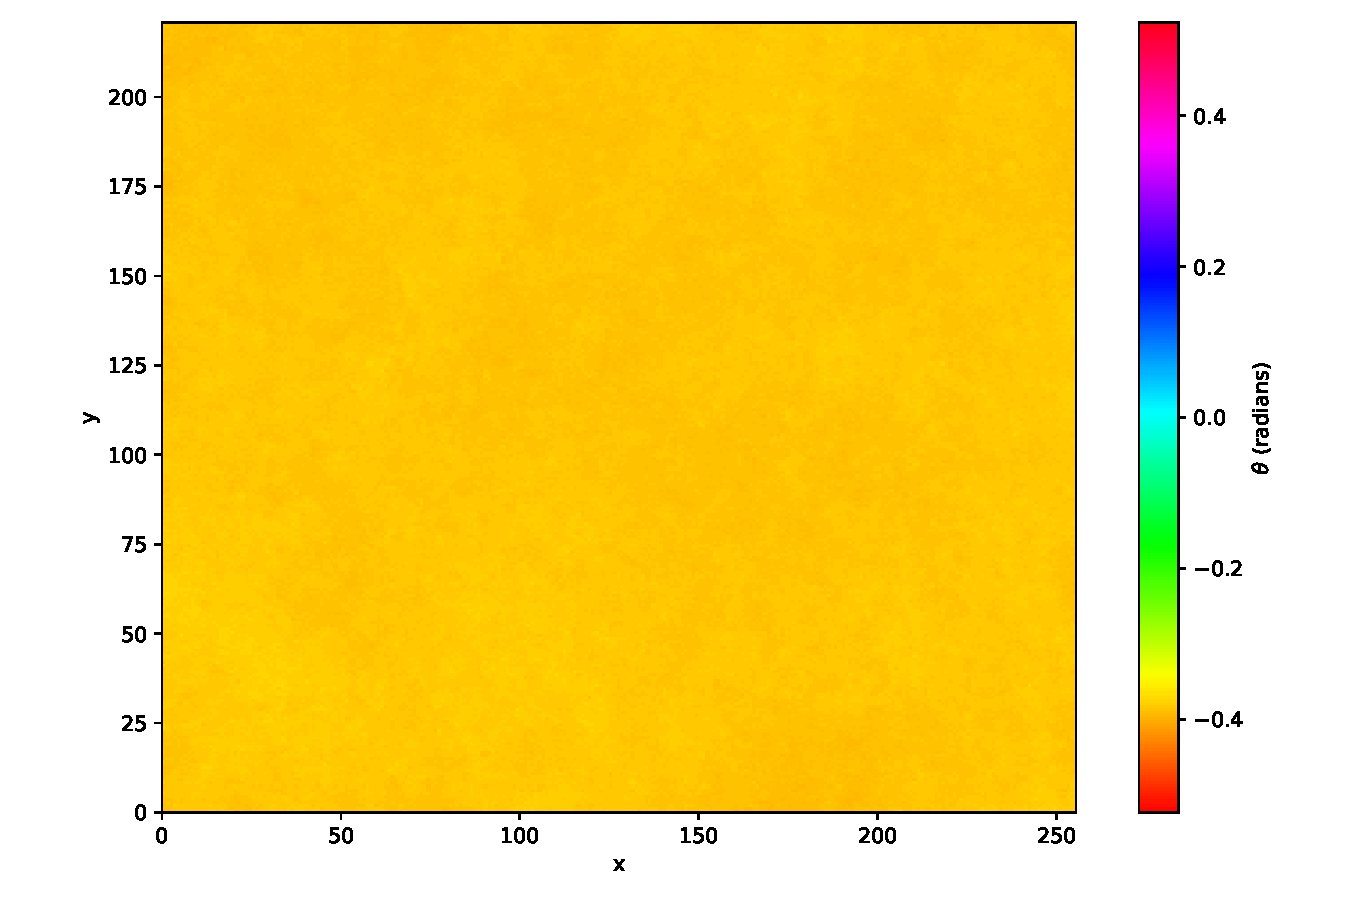
\includegraphics[width=\textwidth]{Figures/gamma1/final_configuration_T1.000e-02_L256.pdf}
        \caption{$T = 0.01$, crystalline phase}
    \end{subfigure}
    \hfill
    \begin{subfigure}[t]{0.495\textwidth}
        \centering
        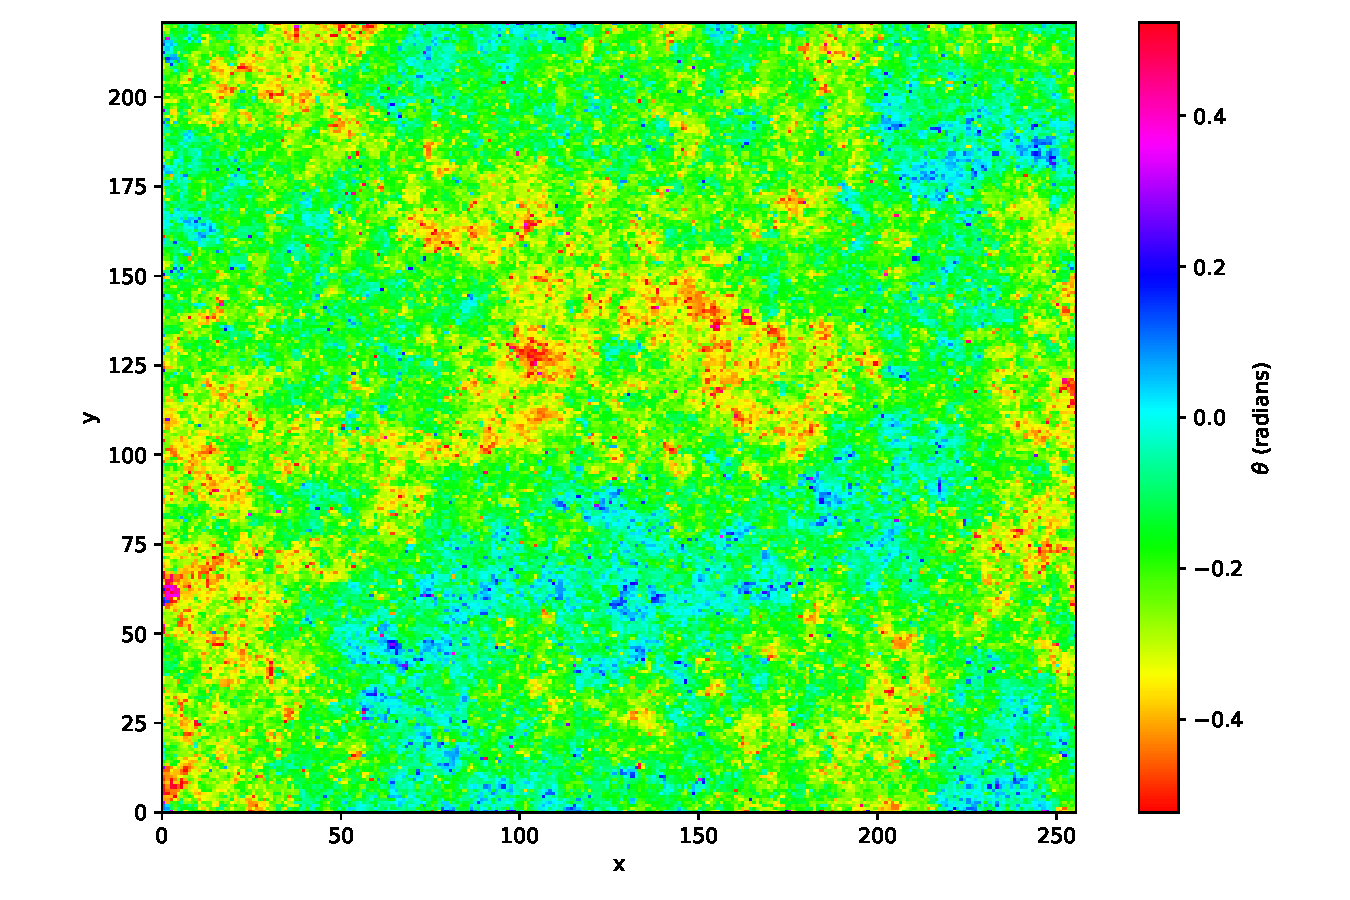
\includegraphics[width=\textwidth]{Figures/gamma1/final_configuration_T1.500e-01_L256.pdf}
        \caption{$T = 0.15$, before transition}
    \end{subfigure}
    
    \medskip

    \begin{subfigure}[t]{0.495\textwidth}
        \centering
        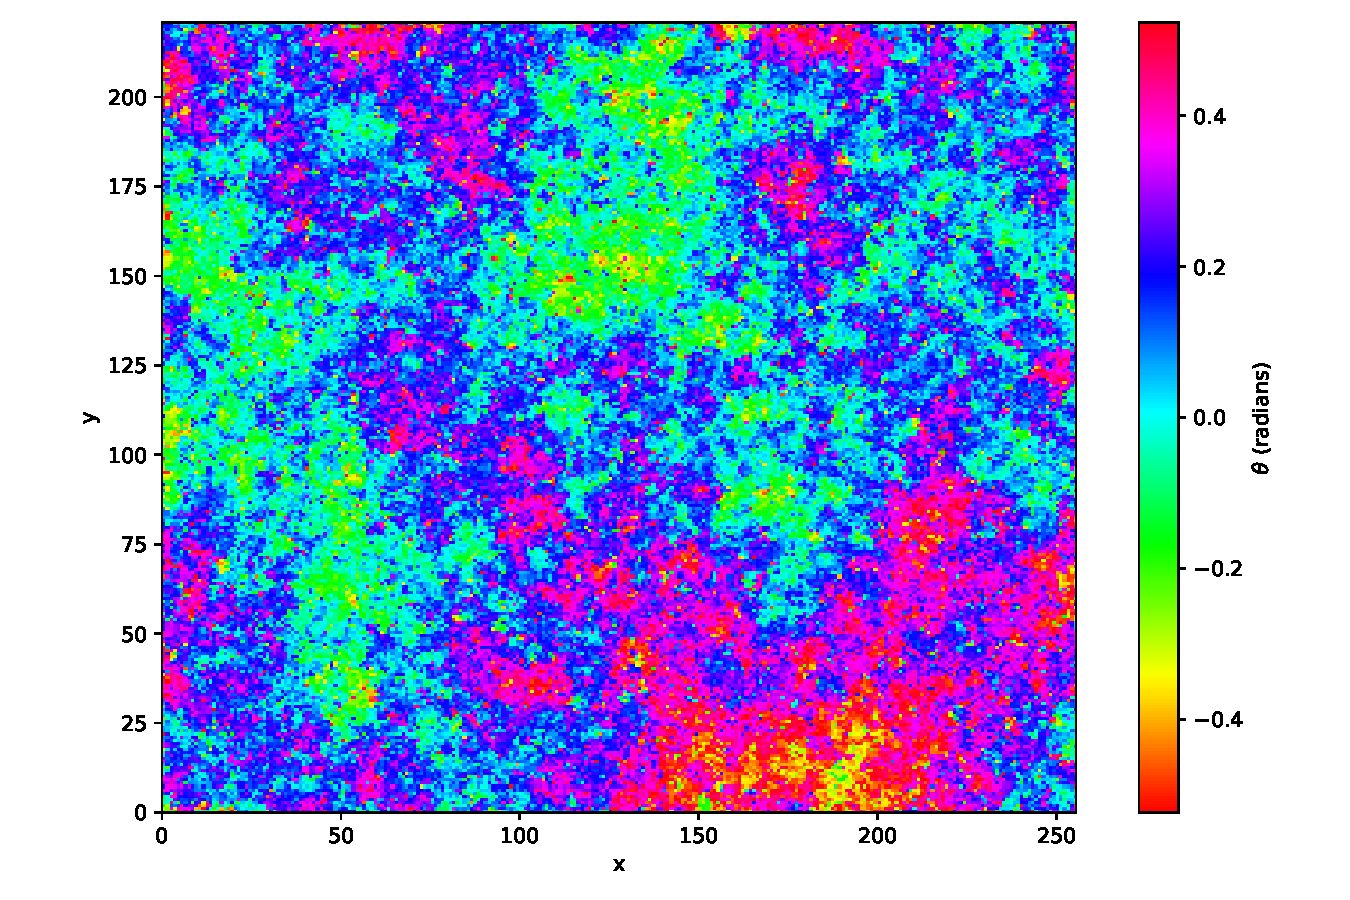
\includegraphics[width=\textwidth]{Figures/gamma1/final_configuration_T1.850e-01_L256.pdf}
        \caption{$T = 0.185$, near transition}
    \end{subfigure}
    \hfill
    \begin{subfigure}[t]{0.495\textwidth}
        \centering
        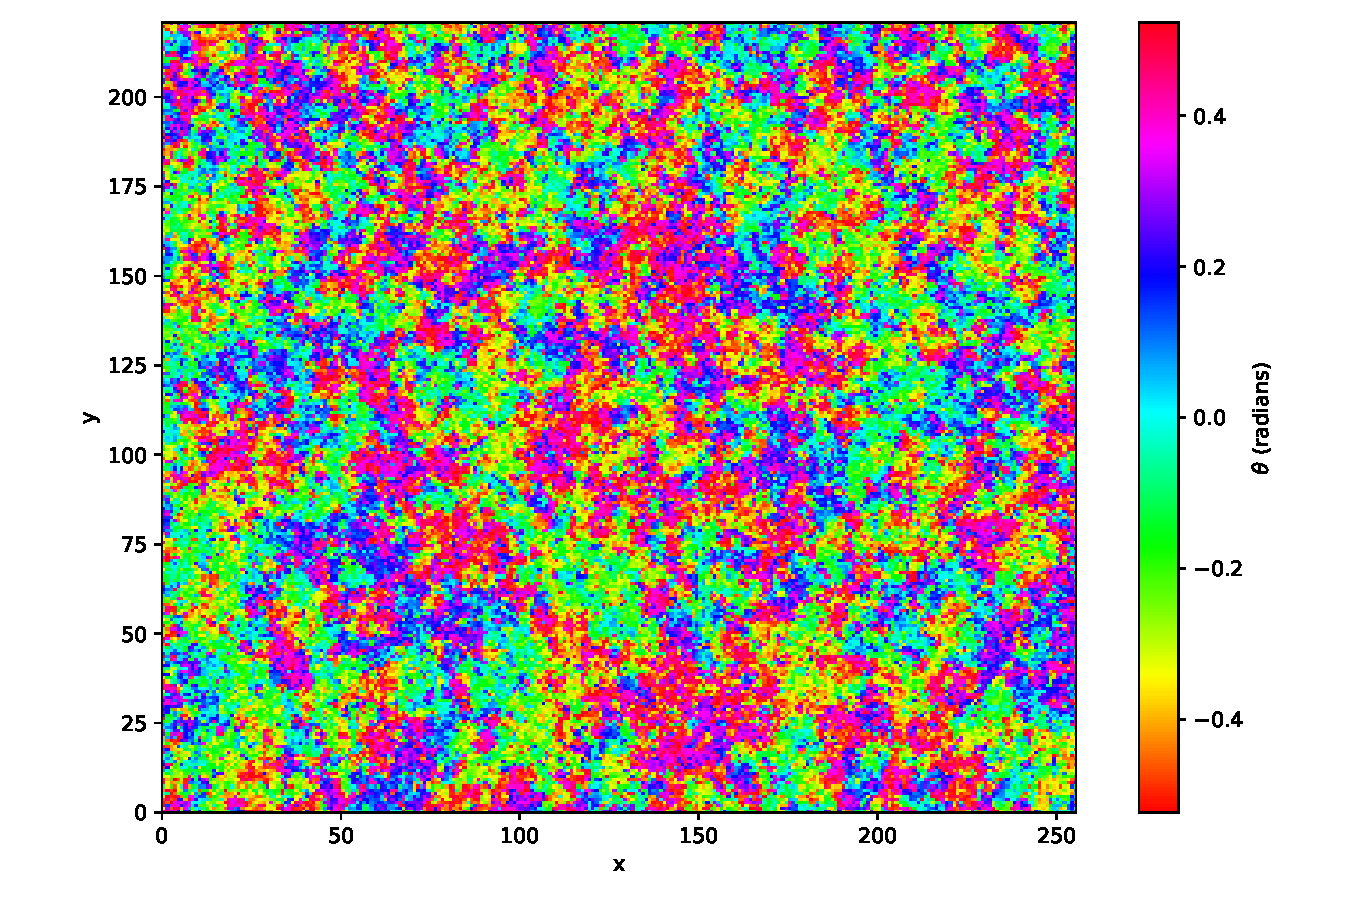
\includegraphics[width=\textwidth]{Figures/gamma1/final_configuration_T2.200e-01_L256.pdf}
        \caption{$T = 0.22$, disordered phase}
    \end{subfigure}
    \caption{Final lattice configurations for the polycrystalline model with $\epsilon = 0.0$ and $\gamma = 1.0$ at different temperatures with lattice size $L = 256$.}
    \label{fig:lattices_eps0_gamma1}
\end{figure}